\chapter{Desarrollo} \label{development}
En este capítulo se presentan las actividades realizadas durante el desarrollo del proyecto correspondientes al período de pasantías Abril-Septiembre 2018. El proyecto inicialmente tenía planteado el desarrollo de cuatro módulos:
\begin{enumerate}
	\item Módulo de administración de cadenas, tiendas, zonas, productos y categorías: En principio el desarrollo de este módulo consistía en el desarrollo de la interfaz gráfica para cada una de estas entidades para la creación, edición y eliminación de registros, sin embargo faltaron las entidades tiendas y zonas, la asignación de tiendas a cadenas, el cual no se realizó, asignar productos a categorías y finalmente crear el listado de los registros de productos con mecanismo de búsqueda.
	\item Módulo de administración de precios: Este módulo incluye la interfaz de creación, edición y eliminación de registros, el desarrollo de un mecanismo para importar los precios en lote usando un archivo en formato Microsoft Excel y de igual manera importar por lote mediante webservice desde una fuente externa en formato JSON, sin embargo ésta última no se realizó.
	\item Módulo de generación de reportes: Para este módulo se planteó el desarrollo de la funcionalidad de generar reportes comparativos para: 
    \begin{itemize}
        \item Gráfico de dispersión de precios / categorías.
        \item Gráfico de barras para un producto seleccionado separando precio normal y oferta.
        \item Gráfico tipo box-plot para el histórico de precios de un producto.
	\end{itemize}
	Implementar un mecanismo automático para generar reportes de manera frecuente y enviar alertas de correo con el resultado, y finalmente un mecanismo para exportar los reportes en un formato tipo tabla en Microsoft Excel, sin embargo estas dos últimas funcionalidades se decidieron dejar para una próxima versión del sistema, ya que el desarrollo de la primera funcionalidad tomó más tiempo del pensado, debido a su complejidad.
	\item Módulo de preferencias para usuario: Este módulo no se desarrolló, debido a que el mismo tenía directa relación con las dos últimas funcionalidades del módulo anterior y al no desarrollarlas, este módulo no tenía sentido. 
\end{enumerate}
    El proyecto se dividió en 3 Fases :
\begin{itemize}
   \item Fase de Inducción, en la cual se hace la introducción del proyecto, el pasante se familiariza con las herramientas y tecnologías necesarias para realizar el proyecto.
   \item Fase de Desarrollo la cual se divide en 5 Sprints, en esta fase se hace la implementación de los diferentes módulos de la aplicación.
   \item Fase de Documentación en la cual se realiza parte de la documentación necesaria para la aplicación.
\end{itemize}
A continuación, se explicará en detalle en qué consiste cada Fase.

\section{Inducción}
Durante esta Fase el pasante realizó un proceso de familiarización con la empresa junto con el estudio de herramientas y lenguajes de trabajo que fueron empleados a lo largo del desarrollo del proyecto.
Realizó varios cursos tutoriales (Umbraco Course level 1, Learn ASP.NET MVC de Microsoft Virtual Academy, entre otros),  y utilizó recursos (guía de Umbraco) que la empresa proporcionó para tener los conocimientos necesarios para llevar a cabo el proyecto. Además investigó sobre herramientas como: ASP.NET, SQL Server, Highcharts y Visual Studio.

La duración de esta fase fue de una semana, sin embargo, el pasante tuvo que mantenerse en constante búsqueda de recursos e investigar sobre la marcha sobre herramientas o conceptos nuevos, los cuales se fueron necesitando en el camino. Todo este proceso fue sumamente útil y de gran aprendizaje ya que la mayoría de las herramientas utilizadas para el desarrollo del proyecto eran nuevas y muchos de los conceptos se investigaron a profundidad.

\section{Desarrollo}
La Fase de desarrollo de la aplicación se realizó en cinco Sprints, los cuales tuvieron una duración en total de 17 semanas continuas. A continuación una descripción del trabajo realizado en cada uno.

\subsection{Primer Sprint}
Durante este Sprint se hizo el análisis y definición de los requerimientos de la aplicación, los cuales eran primero definir el alcance inicial de la aplicación (ver bla bla), definir la arquitectura a utilizar y por último la estructura de la base de datos. El pasante inició la familiarización de la versión actual de CPI junto con el dueño del producto para resolver las posibles dudas de la funcionalidad, o conceptos necesarios para entender la aplicación. Además se creó el repositorio de Git, el proyecto de Visual Studio y el sitio de Umbraco, y por último el Dueño del producto sugirió dos posibles plantillas de HTML que podrían ser utilizadas para las vistas de la aplicación y el pasante eligió la que era más adecuada visual y funcionalmente para la misma. 
\\
\\
\textbf{Actividades realizadas:}
\begin{itemize}
   \item Familiarización con la versión original de CPI. Esta actividad consistió principalmente en reuniones con el dueño del producto para aclarar dudas con respecto a los conceptos necesarios para entender la aplicación y sus funcionalidades.
   \item Elegir la arquitectura de la aplicación. El pasante junto con el Dueño del Producto decidieron utilizar el modelo de 4+1 Vistas de Philippe Kruchten.
   \item Definir los actores del sistema. En principio se definieron dos actores principales para la aplicación, \textit{Admin} (el administrador del sistema) y \textit{Retailer} (representantes de cadenas).
   \item Realizar una matriz de permisología de las funcionalidades de la aplicación. Lo que el pasante realizó fue listar todas las posibles funciones de cada uno de los módulos de aplicación y definir cuáles eran los permisos que tendrán cada uno de los actores.
   \item Elegir las entidades de la aplicación. El pasante basándose en la primera versión de la aplicación y junto el dueño del producto tomaron la decisión de cuáles serían las entidades que se manejarían desde la base de datos de Umbraco (cadenas) y cuáles en la base de datos de SQL Server (tiendas, zonas, productos, precios y categorías).
   \item Rediseñar la base de datos. Luego de decidir cuáles eran las entidades a trabajar en la base de datos de SQL Server el pasante junto con el Dueño del Producto decidieron cuál podría ser la nueva estructura de la base de datos. A continuación se muestra el Diagrama de la versión original de CPI (ver Figura \ref{fig:er_viejo}) y el Diagrama ER de la versión 2 de CPI (ver Figura \ref{fig:er_nuevo})
        \begin{figure}[hbt]
        \begin{center}
        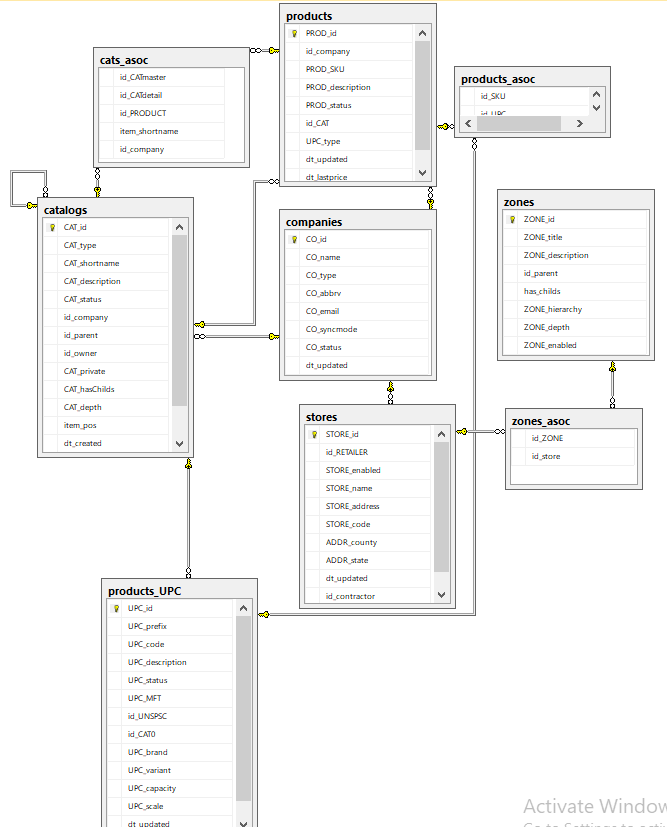
\includegraphics[scale=0.8]{er_viejo.png}
        \caption{Diegrama ER de la base de datos de la versión 1 de CPI.}
        \label{fig:er_viejo}
        \end{center}
        \end{figure}

        \begin{figure}[hbt]
        \begin{center}
        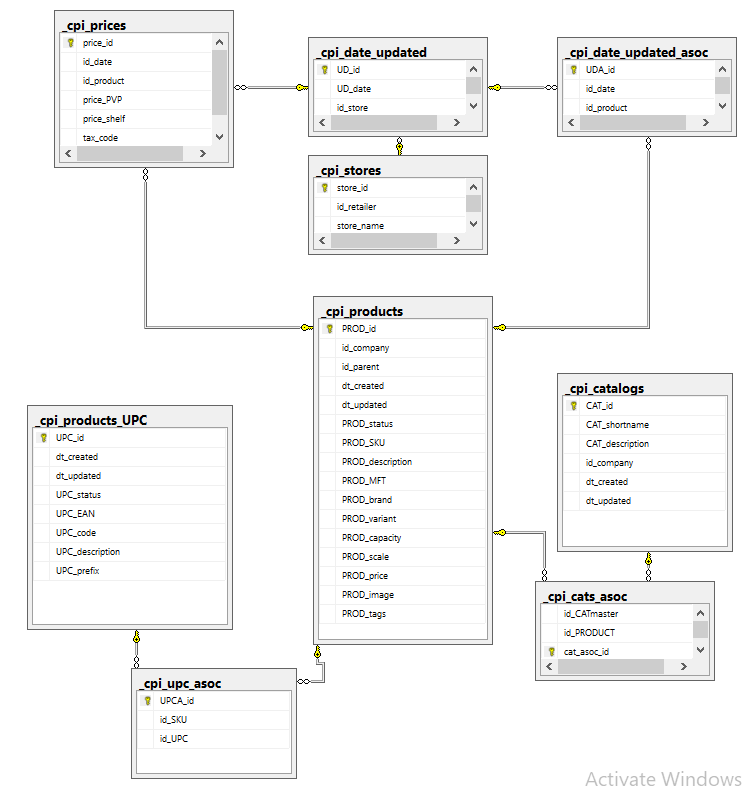
\includegraphics[scale=0.8]{er.png}
        \caption{Diagrama de la base de datos de la nueva versión de CPI.}
        \label{fig:er_nuevo}
        \end{center}
        \end{figure}
        \item Crear el proyecto en Visual Studio. 
        \item Crear el repositorio de Git. Para el proyecto se creó un repositorio llamado CPI el cual se utilizó para el control de versiones del proyecto. Para utilizar correctamente el repositorio el pasante tuvo que refrescar los comandos.
        \item Crear el sitio de Umbraco.
        \item Elegir la plantilla a utilizar para las vistas de la aplicación. El pasante junto con el Dueño del Producto eligieron entre dos posibles plantillas, la elegida fue la que más se acopló a las necesidades de la aplicación.
        \item Investigar sobre Datatables ya que fue el pluggin (complemento) elegido por el Dueño del Producto para manejar dinámicamente las tablas.
        \item Listar las vistas que tendrá la aplicación, según los módulos que se eligieron como alcance inicial.
    \end{itemize}
\textbf{Duración:} 2 semanas.

\subsection{Módulo de Administración de cadenas, productos y categorías (2da Iteración)}
Durante esta iteración se implementó la funcionalidad para el manejo de las principales entidades de la aplicación: cadenas, productos y categorías. En la cual se desarrolló una interfaz gráfica en el back end de Umbraco usando un paquete llamado Fluidity para el manejo de estas entidades en la base de datos. Se definieron los Doctypes y Datatypes para crear el contenido en Umbraco. Se inició el desarrollo de las vistas de la aplicación.

Al finalizar esta iteración fue posible manejar las entidades de la aplicación por medio del árbol de contenido de Umbraco o por medio de la interfaz gráfica de Fluidity. 

\textbf{Actividades realizadas:}
\begin{itemize}
   \item Definir los Doctypes para las entidades principales.
   \item Definir los Datatypes para las entidades principales.
   \item Desarrollar la interfaz de Fluidity para creación, edición y eliminación de registros de las entidades que se guardan en la base de datos de SQL Server.
   \item Iniciar desarrollo de las vistas de la aplicación.
   \item Realizar vista de listado de productos.
\end{itemize}


\textbf{Duración:} 3 semanas.

\subsection{Módulo de Generación de Reportes (3ra Iteración)}
En esta iteración se desarrolló parte de la funcionalidad de generación de reportes comparativos. Se realizó la vista de cada uno de los gráficos (barras y boxplot) que permiten la comparación de precios entre productos de una cadena, o productos que tienen en común distintas cadenas y además tablas que muestran información necesaria para cada uno de estos gráficos. Esta iteración tuvo una duración más larga de la planificada ya que para realizar cada uno de los gráficos se necesitaba traer datos de la base de datos y la traducción del código de la versión antigua a la nueva versión tomó más tiempo de lo esperado ya que no se encontraba bien documentada.


\textbf{Actividades realizadas:}
\begin{itemize}
   \item Desarrollar vista de gráfico de barras para un producto seleccionado de la lista de productos de la cadena, separando precio normal y oferta.
   \item Desarrollar vista de gráfico tipo boxplot para el precio histórico de un producto.
   \item Traducir scripts para traer datos de la base de datos.
   \item Mejorar código y funcionalidad que se desarrollaron en iteraciones anteriores.
\end{itemize}


\textbf{Duración:} 4 semanas.

\subsection{Continuación con el Módulo de Generación de Reportes (4ta Iteración)}
En esta Iteración se siguió el desarrollo de la generación de reportes completando el reporte de precios por categorías (gráfico de dispersión) y se mejoraron algunos aspectos de las otras iteraciones.

\textbf{Actividades realizadas:}
\begin{itemize}
   \item Desarrollar la vista del reporte de precios por categorías.
   \item Mejorar código de la aplicación.
\end{itemize}

\textbf{Duración:} 3 semanas.


\subsection{Refactorización (5ta Iteración)}
Al iniciar esta iteración se llegó a la conclusión que el desarrollo de la funcionalidad que se tenía hasta el momento no estaba siguiendo la estructura que realmente se quería tener en la solución de Visual Studio, ya que los controladores no estaban organizados correctamente según el patrón MVC. Además habian funciones que debían estar implementadas en \verb|CPI_API| pero se encontraba en \verb|CPI_Core| y se estaba utilizando el tipo de controlador incorrecto. Este inconveniente ocurrió por la falta de comunicación entre el dueño del producto y el desarrollador (pasante), sin embargo se hicieron las correcciones necesarias para corregir este imprevisto, sin embargo tomó tiempo extra que no se tenía planificado y por esta razón no se alcanzó a realizar parte de algunos módulos que ya se encontraban en la planificación.


\textbf{Actividades realizadas:}
\begin{itemize}
   \item Reorganizar los controladores de la aplicación.
   \item Refactorizar código en gran parte de la funcionalidad.
   \item Mejorar calidad del código.
\end{itemize}

\textbf{Duración:} 2 semanas.


\subsection{Módulo de Administración de precios (6ta Iteración)}
Esta fue la última Iteración de desarrollo, en la cual se implementó el módulo de administración de precios de productos. Se creó la interfaz gráfica usando Fluidity y además la funcionalidad para importar un lote de precios usando un archivo en formato MS Excel (CSV). Además se hicieron mejoras de código implementado en las iteraciones anteriores y correcciones de bugs.

\textbf{Actividades realizadas:}
\begin{itemize}
   \item Implementar la autenticación, inicio y cierre de sesión para el front end de la aplicación.
   \item Desarrollar interfaz gráfica para creación, edición y eliminación de registros.
   \item Mejorar código y corregir bugs.
\end{itemize}

\textbf{Duración:} 3 semanas.


\section{Documentación} \label{documentation}
Esta última fase del proyecto duró las últimas dos semanas del período de pasantía. Se realizó la documentación necesaria para la aplicación, se dejó expresado el estado final del sistema, se elaboraron los documentos de instalación de CPI y el Documento de Arquitectura de Software donde se detallan los componentes y casos de uso desarrollados de la aplicación.
